\part{Progettazione di un'interfaccia grafica per la compressione di immagini}

L'interfaccia grafica è realizzata con l'ambiente di sviluppo QT\cite{qt}, il quale permette di creare delle GUI scrivendo il codice in linguaggio c++. La compressione applicata è stata limitata solamente alla visualizzazione, ovvero l'immagine perde l'informazione legata alle alte frequenze, però le strutture dati che contengono tale immagine rimangono costanti. Introducendo la possibilità, ad un successivo salvataggio dell'immagine, di memorizzare solamente i coefficienti diversi da 0, richiamando un concetto di simil sparsità però applicato alle frequenze non tagliate dalla compressione.

Il programma fornisce una schermata nella quale è possibile selezionare l'immagine da comprimere e i valori di compressione da applicare, ossia dimensione dei blocchi e la soglia di taglio delle frequenze. Nella parte sinistra della GUI viene mostrata l'immagine originale, mentre in quella di destra la sua versione compressa. In figura\ref{fig:deer} è riportato un esempio sull'immagine \textit{deer}, sulla quale sono stati applicati blocchi di elevate dimensioni (70x70) ed una elevata compressione (circa del 92\%), in questo modo è facilmente osservabile l'effetto della compressione sui blocchi e sull'immagine.

\begin{figure}[h]
	\centering
	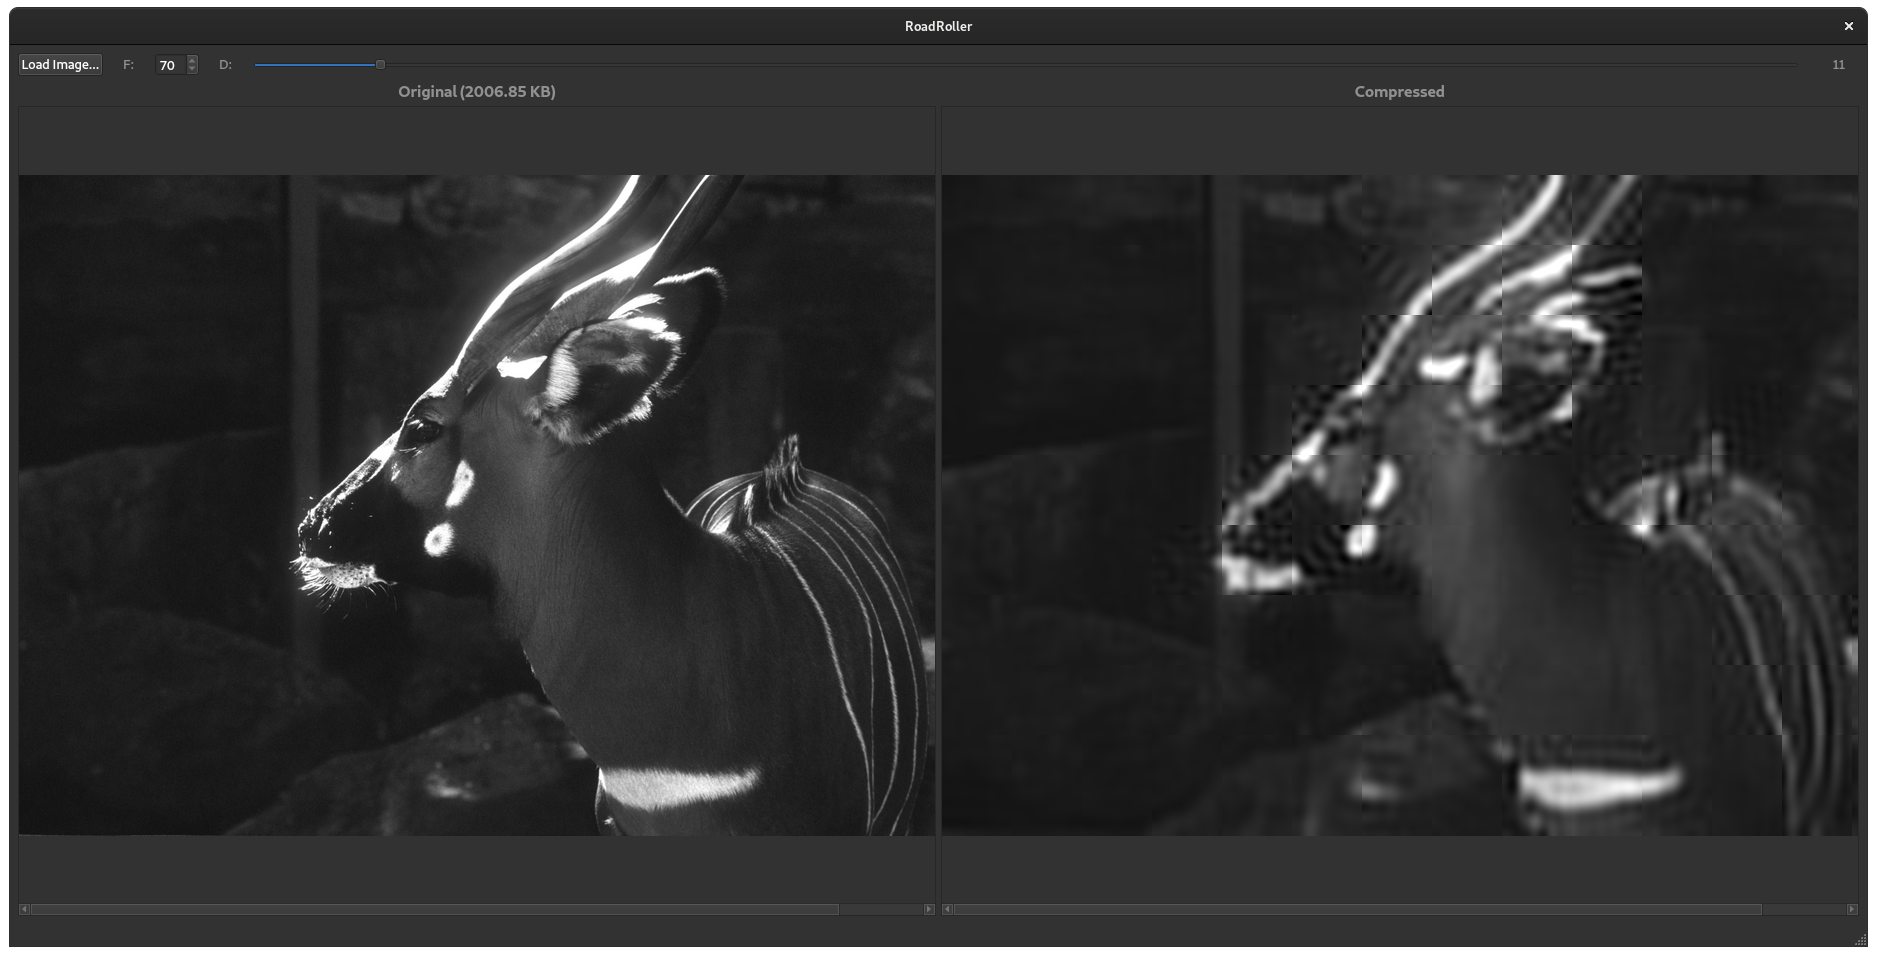
\includegraphics[width=1\linewidth]{figures/qt_deer}
	\caption{Programma di compressione con Qt}
	\label{fig:deer}
\end{figure}

\section{Features}

Alla versione base del progetto, descritto precedentemente, sono state aggiunte un insieme di funzionalità:

\begin{itemize}
	\item \textbf{Multithreading}: L'aggiunta dei thread permette una rapida compressione dell'immagine. Infatti essendo che i blocchi lavorano su aree della figura indipendenti gli uni dagli altri, è possibile eseguire le compressioni in parallelo, così come la scrittura dei pixel nell'oggetto immagine finale.
	\item \textbf{Navigazione dell'immagine}: All'interno dell'interfaccia grafica sono presenti degli slider e dei tasti per zoomare nelle immagine, tali tasti sono sincronizzati in modo tale da poter visionare contemporaneamente le stesse zone delle 2 immagini. In questo modo si possono osservare più comodamente i vari effetti che la compressione comporta sulle immagini.
	\item \textbf{Aggiornamento in tempo reale}: Grazie ai thread, che velocizzano notevolmente il lavoro, modificando la dimensioni dei blocchi e/o la dimensione del taglio delle frequenze, é possibile visionare nella parte di destra gli aggiornamenti sulla compressione, in tempo reale. Il delay che intercorre tra la modifica del parametro e il suo aggiornamento é solitamente molto basso, anche se ovviamente varia in relazione alla dimensione dell'immagine passata in input.
	\item  \textbf{Gestione dei bordi}: Usando blocchi di grandezza variabile, un blocco che si trova sul bordo dell'immagine può includere eventuali pixel esterni, se presenti, in questo modo non si perde informazione sulla risoluzione originale dell'immagine.
\end{itemize}

\section{Dettagli implementativi}

Solitamente é difficile che la dimensione di un blocco sia esattamente un multiplo della risoluzione dell'immagine, per questo motivo i blocchi sui bordi possono avere una dimensione variabile, che gli consente di includere eventuali pixel che verrebbero esclusi.

Questo, anche se non richiesto dalla consegna, ha necessitato la modifica del valore relativo al taglio delle frequenze, per fare in modo che i blocchi definiti sui bordi, gestiscano il taglio delle frequenze su dimensioni rettangolari. In particolare in Figura \ref{fig:taglio} viene mostrato come il taglio di un blocco rettangolare per lo stesso numero, comporta una perdita maggiore di informazioni. Per tale motivo, il valore di qualità per tali blocchi è stato moltiplicato per: \[ dimMassima / blockSize \] dove la \textit{dimMassima} rappresenta il lato più lungo del rettangolo (b in Figura). In questo modo si ottiene il rapporto per scalare correttamente il taglio da una forma quadrata ad una rettangolare.



\begin{figure}
	\begin{minipage}{0.5\textwidth}
		\begin{center}
		
			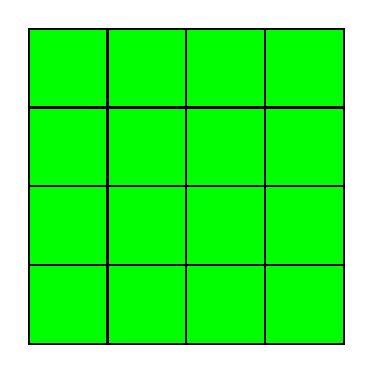
\begin{tikzpicture}
				[%%%%%%%%%%%%%%%%%%%%%%%%%%%%%%
				box/.style={rectangle,draw=black,thick, minimum size=1cm},
				]%%%%%%%%%%%%%%%%%%%%%%%%%%%%%%
				
				\foreach \x in {0,1,...,3}{
					\foreach \y in {0,1,...,3}
					\node[box, fill=red] at (\x,\y){};
				}
			
			
				\foreach \x in {0,...,3}{
					\foreach \y in {0,...,3} {
						\ifnumcomp{\x + (3 - \y)}{<}{5}{
							\node[box, fill=green] at (\x,\y){};
						}{};
					}
				}
				
				
			\end{tikzpicture}
		\end{center}
		\begin{center}
			(a)
		\end{center}
	\end{minipage}\hfill
	\begin{minipage}{0.5\textwidth}
		\begin{center}
			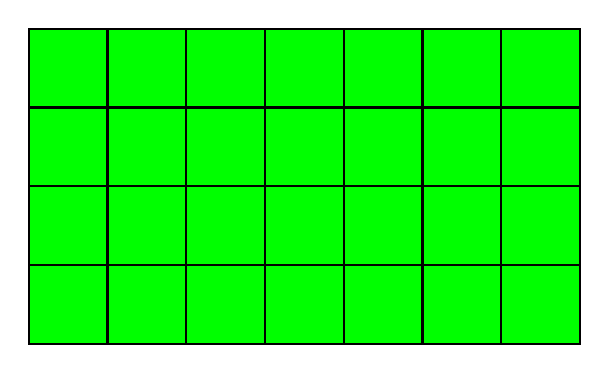
\begin{tikzpicture}
				[%%%%%%%%%%%%%%%%%%%%%%%%%%%%%%
				box/.style={rectangle,draw=black,thick, minimum size=1cm},
				]%%%%%%%%%%%%%%%%%%%%%%%%%%%%%%
				
				\foreach \x in {0,1,...,6}{
					\foreach \y in {0,1,...,3}
					\node[box, fill=red] at (\x,\y){};
				}
				
				
				\foreach \x in {0,...,6}{
					\foreach \y in {0,...,3} {
						\ifnumcomp{\x + (3 - \y)}{<}{5}{
							\node[box, fill=green] at (\x,\y){};
						}{};
					}
				}
				
				
			\end{tikzpicture}
		\end{center}
	\begin{center}
		(b)
	\end{center}
\end{minipage}
\caption{Taglio delle frequenze sulle diverse dimensioni dei blocchi}\label{fig:taglio}
\end{figure}

\section{Visualizzazione dei risultati}

Per mostrare meglio la compressione potremmo momentaneamente ignorare la conversione dei valori tramite la IDCT2. In figura\ref{fig:compression_values} viene mostrato il risultato ottenuto, dove è possibile osservare i coefficienti generati dalla DCT, i quali vengono successivamente tagliati per il valore di input scelto. In questo modo, ogni blocco conterrà dati diversi da 0 solo nella parte superiore del taglio, evidenziata anche graficamente dalla distribuzione del colore bianco nei singoli blocchi. Infatti tale tonalità rappresenta un valore elevato del coefficiente presente nella matrice, mentre le zone nere, rappresentano i valori che sono stati impostati a 0 dal taglio.

\begin{figure}[h]
	\centering
	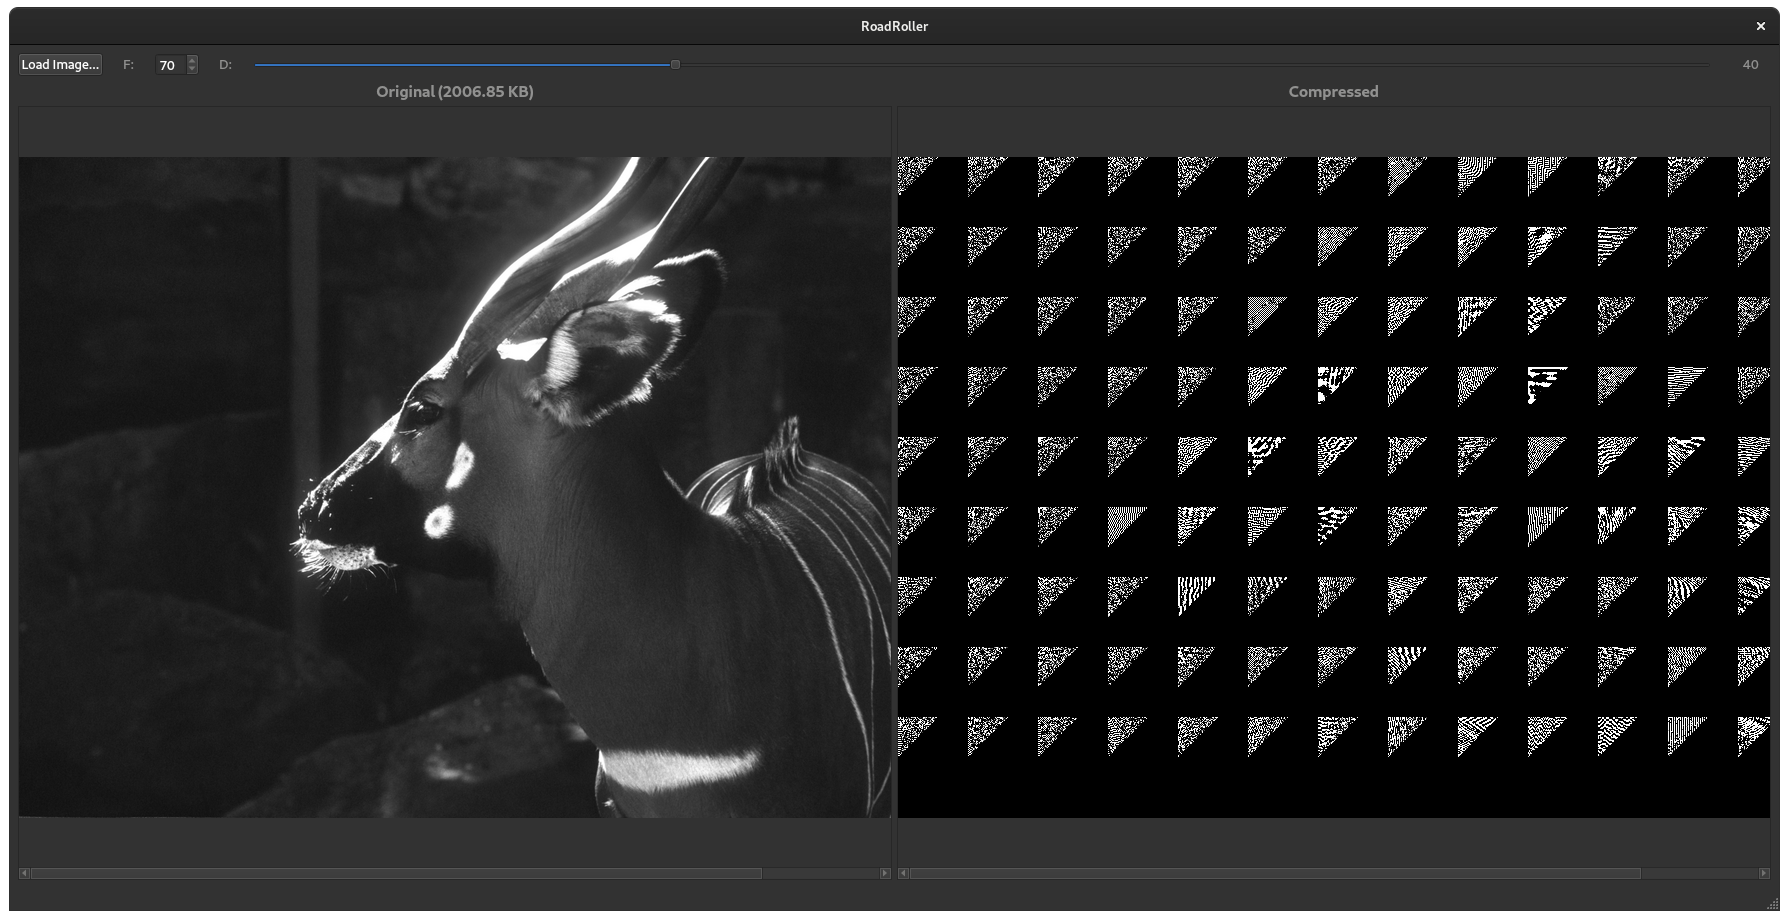
\includegraphics[width=1\linewidth]{figures/qt_dct_values}
	\caption{Valori della DCT generati dalla compressione}
	\label{fig:compression_values}
\end{figure}
